% Mathematics of Computation submission version, revised 1 October 2026.
% Figure 1 is figures/response_difference.pdf, drawn by figures/make_figure_response_difference.py.
% Self-contained AMS-LaTeX manuscript. Compile with pdflatex twice.
\documentclass[10pt]{amsart}
\usepackage[T1]{fontenc}
\usepackage{amssymb,booktabs,array,microtype,graphicx}
\usepackage{algorithm}
\usepackage{algpseudocode}
\usepackage[hidelinks]{hyperref}
\usepackage{cleveref}
\newtheorem{theorem}{Theorem}[section]
\newtheorem{lemma}[theorem]{Lemma}
\newtheorem{proposition}[theorem]{Proposition}
\newtheorem{corollary}[theorem]{Corollary}
\theoremstyle{definition}
\newtheorem{assumption}[theorem]{Assumption}
\theoremstyle{remark}
\newtheorem{remark}[theorem]{Remark}
\newcommand{\R}{\mathbb R}
\newcommand{\C}{\mathbb C}
\newcommand{\E}{\mathbb E}
\newcommand{\Prob}{\mathbb P}
\newcommand{\eps}{\varepsilon}
\newcommand{\dd}{\,d}
\newcommand{\Mplus}{\mathcal M_+(J)}
\newcommand{\ThetaAll}{\Theta_+}
\newcommand{\F}{\mathcal F}
\newcommand{\Pp}{\mathcal P}
\newcommand{\Tclass}{\mathcal T_{\boldsymbol s}}
\newcommand{\Teff}{\mathcal T_{\boldsymbol s}^{\mathrm{eff}}}
\newcommand{\Rclass}{\mathcal R_{\boldsymbol r}}
\newcommand{\norm}[1]{\left\|#1\right\|}
\newcommand{\abs}[1]{\left|#1\right|}
\newcommand{\supp}{\operatorname{supp}}
\newcommand{\KL}{\operatorname{KL}}
\newcommand{\kl}{\operatorname{kl}}
\newcommand{\TV}{\operatorname{TV}}
\newcommand{\doi}[1]{\href{https://doi.org/#1}{doi:\nolinkurl{#1}}}

\title[Frequency saturation and certified computation]{Frequency Saturation and Certified Computation of Relaxation Functionals}
\author{Haotian Zhong}
\address{Department of Mathematics, School of Sciences, Shanghai University, Shanghai 200444, P. R. China}
\email{zhonghaotian1219@gmail.com}
\thanks{ORCID: \href{https://orcid.org/0009-0009-5567-1315}{0009-0009-5567-1315}.}
\subjclass[2020]{Primary 65J22, 65Y20; Secondary 65G20, 62L12, 62G15}
\keywords{Positive measures, inverse problems, information complexity, frequency sampling, verified computation, sequential stopping}
\date{}
\hypersetup{pdftitle={Frequency Saturation and Certified Computation of Relaxation Functionals},pdfauthor={Haotian Zhong}}
\begin{document}
\begin{abstract}
Impedance measurements of a relaxing medium follow a Stieltjes-type law $Z(\omega)=R+i\omega L+\int(1+i\omega\tau)^{-1}\,d\mu(\tau)$, where $\mu$ is a positive measure of relaxation times on a compact interval and the resistance $R$ and inductance $L$ are unknown nonnegative calibration parameters. We ask how much frequency information is needed to compute a linear functional $\int f\,d\mu$ of the measure, and how to compute, with certified numerical error, the complete range of values consistent with noisy data. Four results are established. Exactly $K+2$ distinct frequencies are necessary and sufficient for uniform noiseless identification of every reference measure with at most $K$ atoms among all finite positive measures when $R$ and $L$ are unknown, and $K+1$ when they are known. This minimal design already attains, up to constants, the worst-case accuracy of the entire positive-frequency response: for a target of regularity $s_j$ near a cluster of $r_j$ reference atoms the sharp exponent is $\min\{1,s_j/(2r_j)\}$, uniformly through colliding atoms and vanishing masses. Positive moment-matched pairs that stay close at every frequency give the lower bound, and polynomial reproduction that annihilates the calibration parameters gives the upper bound. On strictly feasible rational observation boxes, a finite exact-arithmetic refinement algorithm encloses both endpoints of the continuous data-consistent range with any prescribed numerical excess, and computable width brackets yield absolute--relative stopping criteria. The same modulus determines the optimal expected measurement effort for a terminal interval of width $w$ and confidence $1-\alpha$ under a Gaussian variance--effort model, allowing adaptive frequency, precision, and stopping rules; a class-tuned expanding design that invokes the certified range computation attains this order and terminates almost surely at every finite positive spectrum. Exact certificates and executed stopping paths accompany the results.
\end{abstract}
\maketitle

\section{Introduction}\label{sec:intro}
\subsection{The problem}
Impedance spectroscopy records the complex response $Z(\omega)$ of an electrochemical or dielectric system at a finite set of angular frequencies~\cite{orazem}. For a large class of systems the response is a superposition of first-order relaxation processes, each with its own relaxation time, and the standard representation is
\[
 Z(\omega)=R+i\omega L+\int\frac{d\mu(\tau)}{1+i\omega\tau},
\]
where the positive measure $\mu$, the \emph{distribution of relaxation times}, carries the physical information, while the ohmic resistance $R\ge0$ and the inductance $L\ge0$ are calibration parameters that are rarely known exactly. Recovering $\mu$ from noisy samples of $Z$ is a severely ill-posed inverse problem of Stieltjes type~\cite{grabovsky,browngrabovsky}; in practice it is treated by regularized inversion~\cite{ciucci,wan}, which returns one plausible spectrum. The quantities that are eventually reported, however, are usually integrals of the spectrum rather than its individual atoms: the total polarization resistance $Z(0)-R$ is the total mass of $\mu$, and the contribution of the processes in a window of relaxation times is the integral of a smoothed window function. For such a linear functional $F_f(\mu)=\int f\dd\mu$ three concrete questions arise. How many distinct frequencies are needed in principle? How much measurement effort is needed to reach a prescribed accuracy? And how can the complete range of functional values consistent with the data be computed with a rigorous bound on the numerical error?

This paper answers the three questions for the normalized model
\[
 Z_\vartheta(\omega)=R+i\omega L+\int_J\frac{d\mu(x)}{1+i\omega t(x)},\qquad \vartheta=(\mu,R,L),
\]
in which $t(x)=1+x/2$ maps $J=[-1,1]$ onto the relaxation-time interval $[1/2,3/2]$, $\mu$ is an arbitrary finite nonnegative Borel measure on $J$, and $R,L\ge0$. The normalization is a convenience: the proofs use the compactness of the relaxation-time interval and the positivity of its left endpoint, and the constants depend on them. A design $\Omega$ of $m$ distinct positive frequencies yields $2m$ real observations, the real and negative imaginary parts of $Z_\vartheta(\omega_i)$, each known up to a componentwise error bound $\delta$. The data determine the set of all triples consistent with the observations and, for a continuous target $f$, the range $[L_f,U_f]$ of $F_f$ over that set. Its width $W_f=U_f-L_f$ is the \emph{information width}: no method can guarantee better accuracy from these data. The computational task is to return an interval that contains $[L_f,U_f]$ and whose \emph{numerical excess}, its width minus $W_f$, is below a prescribed tolerance. Performance is measured uniformly over sparse references with at most $K$ atoms, while every enclosure and every coverage statement holds over all finite positive measures, including spectra with more atoms than the reference.

\subsection{Main results}
The central result connects a minimal identifying design, a sharp information modulus, and certified range computation. A finite design attains the accuracy order available from the entire positive-frequency response, the same modulus determines the acquisition effort needed for a requested output width, and the computational construction preserves the original observation inequalities while certifying finite optimization, target approximation, and continuous-domain errors separately.

\paragraph{Minimal design and sharp information order.}
We prove that $K+2$ distinct complex frequencies are the minimum required for uniform noiseless identification of references with at most $K$ atoms when resistance and inductance are unknown. Every design at or above this threshold identifies every such reference among all finite positive measures. Below it, references with positive interior atoms and positive calibration values admit exact positive-measure alternatives with a different smooth-functional value. Knowing both calibration values reduces the threshold to $K+1$ (Proposition~\ref{prop:frequencycount}).

The identifying design also attains the sharp noisy recovery order. For a global $C^s$ target ball, the worst-case functional diameter over the class is $\Theta(\eps^\gamma)$, where $\gamma=\min\{1,s/(2K)\}$, both for $K+2$ fixed frequencies and for the entire positive-frequency response. A localized form resolves different regularities near different clusters. If cluster $j$ contains at most $r_j$ reference atoms and the target has regularity $s_j$ there, put
\begin{equation}\label{eq:rates-summary}
 \beta_j=\min\{1,s_j/(2r_j)\},\qquad
 \Psi(v)=v+\sum_jv^{\beta_j},\qquad \beta=\min_j\beta_j.
\end{equation}
Positive moment-matched spectra remain close at every admissible frequency and realize the lower order. Finite-design polynomial reproduction gives the matching upper order. These two constructions establish frequency saturation and give lower bounds against target-aware adaptive frequency queries (Theorem~\ref{thm:saturation}). Proposition~\ref{prop:operator} identifies the sufficient operator properties, and Corollary~\ref{cor:global} treats the standard global target class. The constants are uniform through vanishing masses and colliding reference atoms for each fixed observation design.

\paragraph{Certified computation at the information scale.}
For each strictly feasible rational observation box, a finite exact-arithmetic refinement computes an outer enclosure of the entire continuous functional range with at most $\tau$ additional width (Theorem~\ref{thm:numerical}). A mass-direction correction converts node-dual witnesses into continuous certificates, and finite budgets ensure progress through unsuccessful nonnegativity checks. Positive, mean-preserving projection provides a quadratic strict-feasibility guard. The resulting certificates also give a lower bracket for the true information width and hence an absolute--relative stopping rule (Corollary~\ref{cor:relative}). Algorithm~\ref{alg:range} states the refinement procedure explicitly. Thus the accuracy of the reported range is certified against the original infinite-dimensional problem, not against a discretization of it. In the executed examples of Table~\ref{tab:stopping}, the certified ranges exceed the information width by less than $2\%$.

\paragraph{Attainable acquisition complexity.}
In a Gaussian precision model, a complex observation of effort $a$ has independent real-channel variances $\sigma^2/a$ and costs $a$. For terminal interval width $w$ and coverage $1-\alpha$ over all finite positive spectra, we establish
\begin{equation}\label{eq:cost-summary}
 \mathcal C^*(w,\alpha)\asymp\sigma^2w^{-2/\beta}\log(1/\alpha).
\end{equation}
The lower bound permits adaptive choices of frequency, precision, and stopping. A predetermined expanding design tuned to the specified reference and target class attains this order by invoking the certified range calculation. The same procedure completes almost surely, with pointwise finite expected acquisition count, at every fixed finite positive spectrum (Theorem~\ref{thm:cost} and Proposition~\ref{prop:complete}). The matched resource is measurement effort. Numerical certification supplies a separate, finite computation of the terminal range.

These results distinguish three design decisions: how many distinct frequencies identify the reference, how much measurement effort resolves the target, and how tightly the resulting range is computed. The numerical evidence follows the same division. Exact noiseless alternatives check the identification threshold; all-frequency certificates and equal-effort comparisons examine information limits and design constants; verified stopping paths exercise the range algorithm and its acquisition interface.

\subsection{Relation to existing work}
Extremal problems for linear functionals of positive measures under finitely many moment-type constraints are classical: the Markov--Krein theory of Chebyshev systems~\cite{karlinstudden,kreinnudelman} determines the exact range of $\int f\dd\mu$ when finitely many generalized moments are known exactly. Here the constraints are noisy, componentwise, and carry two unknown calibration coordinates, and the quantity computed is the range over all positive measures consistent with the data. Continuous primal--dual range inference~\cite{stark}, computational optimal recovery~\cite{ettehad}, deterministic-to-statistical moduli~\cite{donoho}, and honest intervals on local performance classes~\cite{cailow} provide the foundations for recovering a functional from such incomplete data. Brown and Grabovsky~\cite{browngrabovsky} establish sharp extrapolation exponents and local extremality conditions for completely monotone functions under relative $L^2$ discrepancy; their extrapolated value is a linear functional of a representing positive measure. Here componentwise RC observations lead to a sharp comparison of finite designs, the full frequency axis, and sequential acquisition. The distribution of relaxation times is routinely estimated from impedance data by regularized inversion~\cite{ciucci,wan}; those methods return one regularized spectrum, whereas the present analysis quantifies what any method can guarantee about an integral of the spectrum and computes that guarantee.

Positive-measure uniqueness in Chebyshev systems is established by Eftekhari et al.~\cite[Proposition~8]{eftekhari}. Proposition~\ref{prop:frequencycount} determines the exact frequency count for RC observations with two conic calibration coordinates. Wu and Yang~\cite[Proposition~5]{wuyang} and Nguyen et al.~\cite[Theorem~5 and Appendix~A.6]{nguyen} develop cluster-sensitive moment and mixture geometry. We use these interpolation principles to obtain spatially varying target-regularity moduli and pair them with positive alternatives that are uniformly close across the entire measurement family. Remark~\ref{rem:fourier} distinguishes the uniform smoothing of the RC kernel from the bandwidth dependence of positive Fourier super-resolution~\cite{liuammari}.

Comparing restricted and richer information classes is a central problem in computational approximation. Wasilkowski and Wo\'zniakowski~\cite{wasilwoz} compare randomized function-value information with worst-case linear information for multivariate approximation in reproducing kernel Hilbert spaces and construct algorithms attaining the corresponding convergence rates. General adaptive-information comparisons~\cite{knu} and noisy-information bounds through entropy numbers~\cite{knpu} further identify the role of information classes and normalization. In the present inverse problem, admissible information consists of RC evaluations; an explicit all-frequency response pair and a finite reproducing design yield the matching orders. Stieltjes reconstruction~\cite{grabovsky} and circuit-parameter frequency design~\cite{sovljanski} provide complementary perspectives, and Section~\ref{sec:experiments} quantifies constant-factor differences between designs on the same positive pair.

Stopped change of measure~\cite{castro,kaufmann,garivier} and time-uniform coverage~\cite{howard} supply the sequential information tools. Polynomial semi-infinite optimization~\cite{papp}, continuous exchange refinement~\cite{grid}, and verified finite optimization~\cite{jansson,schmid} supply computational foundations. The contribution here is the sharp calibrated information law together with an attaining acquisition design and a finite, accuracy-controlled computation of the same continuous feasible range. The original-coordinate error accounting makes these parts one computational recovery problem.

\subsection{Organization and notation}
Section~\ref{sec:model} fixes the model, the reference and target classes, and the two widths. Section~\ref{sec:pair} constructs positive pairs that are close at every frequency and gives the exact response identity behind all lower bounds. Section~\ref{sec:diameter} proves the local modulus, the saturation theorem, the operator conditions, the global corollary, and the exact identification count. Section~\ref{sec:cert} develops the continuous range certification and Algorithm~\ref{alg:range}. Section~\ref{sec:sequential} proves the acquisition law and the all-model completion. Section~\ref{sec:experiments} reports the exact certificates, Tables~\ref{tab:efficiency}--\ref{tab:guard}, and Figure~\ref{fig:pairs}; Section~\ref{sec:conclusions} concludes.

Throughout, $J=[-1,1]$, $t(x)=1+x/2$, $\Mplus$ is the cone of finite nonnegative Borel measures on $J$, $\ThetaAll=\Mplus\times\R_+^2$, and $F_f(\mu)=\int f\dd\mu$. $\Pp_n$ denotes the real polynomials of degree at most $n$, and $\|p\|_{\mathrm{coeff},1}$ is the $\ell^1$ norm of the monomial coefficients of $p$. $\|\cdot\|_\infty$ is the supremum norm on $J$ or on $(0,\infty)$, or the maximum norm on $\R^{2m}$, as the context indicates, and $\|\cdot\|_1$ is the $\ell^1$ norm. A pair $(\mu,\theta)$ is \emph{raw feasible} if it satisfies the original componentwise observation inequalities \eqref{eq:raw}. Constants $c,C$ are positive, may change from line to line, and depend only on the quantities listed in Section~\ref{sec:model}; $\asymp$ and $\Theta(\cdot)$ denote two-sided bounds with such constants.

\section{Model, target classes, and information ranges}\label{sec:model}
This section fixes the observation model, the reference and target classes over which performance is measured, and the two widths, information width and numerical excess, that the later sections bound. Let $J=[-1,1]$, $t(x)=1+x/2$, and
\begin{equation}\label{eq:model}
 \begin{aligned}
 k_\omega(x)&=\frac1{1+i\omega t(x)},\\
 Z_\vartheta(\omega)&=R+i\omega L+\int_J k_\omega(x)\dd\mu(x),
 \quad\vartheta=(\mu,R,L)\in\ThetaAll:=\Mplus\times\R_+^2.
 \end{aligned}
\end{equation}
Here $\Mplus$ denotes finite nonnegative Borel measures. A complex observation gives its real and negative imaginary parts. For a finite design $\Omega=(\omega_1,\ldots,\omega_m)$, write the real observation vector as $A_\Omega\mu+B_\Omega\theta$, $\theta=(R,L)$, where the two rows at $\omega_i$ are
\[
 \phi_{i,R}(x)=\frac1{1+\omega_i^2t(x)^2},\quad
 \phi_{i,I}(x)=\frac{\omega_it(x)}{1+\omega_i^2t(x)^2},\quad
 B_{i,R}=(1,0),\quad B_{i,I}=(0,-\omega_i).
\]
For a real continuous target $f$, let $F_f(\mu)=\int f\dd\mu$. Original componentwise bounds define
\begin{equation}\label{eq:raw}
 \F_\Omega(y,\delta)=
 \{(\mu,\theta)\in\ThetaAll:|A_\Omega\mu+B_\Omega\theta-y|\le\delta\}.
\end{equation}
For a nonempty such set let $L_f,U_f$ be the infimum and supremum of $F_f$ and $W_f=U_f-L_f$. The quantity $W_f$ is the data-induced information width; numerical excess is the additional width of a computed enclosure.

Fix disjoint, nondegenerate closed core intervals $I_j$ in the interior of $J$ and disjoint padded open intervals $V_j\supset I_j$. Their gaps and core-to-boundary distances have a fixed positive lower bound. Integers $r_j\ge1$ satisfy $\sum_{j=1}^qr_j=K$. The reference class is precisely
\[
 \Rclass=\left\{\sum_{j=1}^q\sum_{\ell=1}^{r_j}p_{j\ell}\delta_{c_{j\ell}}:
 p_{j\ell}\ge0,\ \sum_{j,\ell}p_{j\ell}=1,\ c_{j\ell}\in I_j\right\}.
\]
The class includes zero weights and repeated nodes, with reference support contained in the union of the cores. Competitors in \eqref{eq:raw} remain unrestricted positive measures on $J$. For $0<s_j\le2K$, define
\begin{equation}\label{eq:targets}
 \Tclass=\{f\in C(J):\|f\|_\infty\le1,\ 
          \|f\|_{C^{s_j}(V_j)}\le1\text{ for all }j\}.
\end{equation}
Integer norms bound all derivatives through the indicated order. For $s=k+\gamma$, $0<\gamma<1$, they also bound the $\gamma$-H\"older seminorm of the $k$th derivative. Only continuity is required between the pads. The analytical class $\Tclass$ includes all such functions. Algorithmic assertions use $\Teff$, whose members are supplied with certified rational-point evaluations and a computable modulus of continuity. The fixed class data are effectively specified, including a certified bound for the constant in Theorem~\ref{thm:modulus} when a class-tuned cost is asserted. Smooth rational constructions (and normalized effective bumps) give the same lower orders in $\Teff$. The acquisition criterion charges observation effort; target evaluation and arithmetic are separate computational resources.

Constants may depend on $K$, the fixed cores and pads, target orders, and a fixed distinct-frequency design. They are independent of the noise scale, requested width, individual atom masses, within-core distances, and reference nuisance coordinates. The observation design and the compact interval of strictly positive relaxation times are fixed in these uniform bounds. Since the number of cores is fixed, the sum in \eqref{eq:rates-summary} is comparable to its largest term for small $v$.

\begin{remark}[Coverage and local performance]\label{rem:coverage}
Performance is evaluated on $\Rclass\times\Tclass$, while certification and statistical coverage hold on the entire positive cone $\ThetaAll$. This cone includes arbitrary finite masses and spectra with more than $K$ atoms. In particular, the lower constructions compare $r$ reference atoms with $r+1$ alternative atoms in a core. The defining worst-class supremum is taken separately at each noise level, so the maximizing reference and target may vary with that level.
\end{remark}

\section{Positive pairs that are close at every frequency}\label{sec:pair}
All lower bounds in this paper come from pairs of positive measures whose responses differ by $O(h^{2r})$ at \emph{every} frequency while a smooth target separates them at the scale $h^{s}$. This section constructs such pairs explicitly. The mechanism is the uniform smoothing of the RC kernel: because the relaxation times are bounded away from zero, the $x$-derivatives of the kernel are bounded uniformly in the frequency, so a moment-matched signed combination of point masses has a small response everywhere. Proposition~\ref{prop:identity} gives the exact response difference of the pair and locates its unique maximizing frequency, which is the quantity certified in Section~\ref{sec:experiments}. We begin with the derivative bound.
\begin{lemma}[Uniform smoothing]\label{lem:derivative}
For every integer $d\ge1$,
\begin{equation}\label{eq:derivative}
 \sup_{\omega>0}|\partial_x^dk_\omega(x)|
 =\frac{d!}{(2t(x))^d}\frac{d^{d/2}}{(d+1)^{(d+1)/2}}
 \le d!.
\end{equation}
\end{lemma}
\begin{proof}
Differentiation gives $d!(\omega/2)^d/(1+\omega^2t^2)^{(d+1)/2}$. With $z=\omega t$, the logarithmic derivative of the frequency factor is $d/z-(d+1)z/(1+z^2)$, which changes sign only at $z=\sqrt d$. Substitute this maximum and use $2t\ge1$.
\end{proof}

For $r\ge1$, choose $c\in\R,h>0$ with $x_\ell=c+(\ell-r)h\in J$, $0\le\ell\le2r$, and put
\begin{equation}\label{eq:pair}
 \mu_0=2^{-(2r-1)}\sum_{\substack{0\le\ell\le2r\\\ell\text{ odd}}}\binom{2r}{\ell}\delta_{x_\ell},
 \qquad
 \mu_1=2^{-(2r-1)}\sum_{\substack{0\le\ell\le2r\\\ell\text{ even}}}\binom{2r}{\ell}\delta_{x_\ell}.
\end{equation}
Both measures are probabilities; they have $r$ and $r+1$ atoms, respectively, and identical moments through degree $2r-1$.

\begin{proposition}[Exact response difference]\label{prop:identity}
For identical nuisance coordinates and $t_\ell=t(x_\ell)$,
\begin{equation}\label{eq:identity}
 \Delta Z(\omega)=\frac{(2r)!(i\omega h/2)^{2r}}
 {2^{2r-1}\prod_{\ell=0}^{2r}(1+i\omega t_\ell)},\qquad
 \|\Delta Z\|_{\infty,(0,\infty)}\le\frac{(2r)!}{2^{2r-1}}h^{2r}.
\end{equation}
Its squared modulus has a unique positive maximizer $v_*=\omega_*^2$, characterized by
\begin{equation}\label{eq:maximizer}
 \sum_{\ell=0}^{2r}\frac{t_\ell^2v_*}{1+t_\ell^2v_*}=2r,
 \qquad \frac{2r}{t_{\max}^2}\le v_*\le\frac{2r}{t_{\min}^2}.
\end{equation}
For fixed $r,c$, $\omega_*\to\sqrt{2r}/t(c)$ as $h\downarrow0$.
\end{proposition}
\begin{proof}
The elementary identity
\[
 \sum_{\ell=0}^n\frac{(-1)^\ell\binom n\ell}{a+\ell b}
 =\frac{n!b^n}{\prod_{\ell=0}^n(a+\ell b)}
\]
follows by multiplication by the common denominator. Apply it with $n=2r$, $a=1+i\omega t_0$, $b=i\omega h/2$. The uniform bound follows by expressing the forward difference as the integral of a $2r$th derivative over $[0,h]^{2r}$ and using Lemma~\ref{lem:derivative}. The squared modulus is $C_{r,h}v^{2r}/\prod(1+t_\ell^2v)$, where $C_{r,h}=((2r)!)^2h^{4r}/2^{8r-2}$. Its logarithmic derivative times $v$ is $2r-\sum t_\ell^2v/(1+t_\ell^2v)$. The sum increases strictly from zero to $2r+1$, proving uniqueness and the bracket. The bracket converges to $2r/t(c)^2$.
\end{proof}

This exact resolvent identity turns the moment-matched positive pair into a full-frequency information certificate, with a computable response supremum. A target bump centered at an extreme even node, with support radius less than $h/2$ and amplitude proportional to $h^s$, vanishes on $\mu_0$ but has integral at least $c_sh^s$ on $\mu_1$. Scaled smooth bumps have uniformly bounded $C^s$ or H\"older norms, including fractional $s$. Thus the same positive pair combines response scale $h^{2r}$ with target scale $h^s$.

\begin{remark}[Why unlimited Fourier bandwidth is different]\label{rem:fourier}
For the kernel $e^{i\omega x}$ the corresponding normalized difference has modulus $|1-e^{i\omega h}|^{2r}/2^{2r-1}$, equal to $2$ at $\omega h=\pi$. Increasing Fourier bandwidth can therefore expose this pair at order one. The comparison isolates uniform smoothing \eqref{eq:derivative} as the mechanism behind the RC absolute-error saturation result.
\end{remark}

\section{Local moduli and full-frequency saturation}\label{sec:diameter}
This section proves the matching upper bounds and combines them with the pairs of Section~\ref{sec:pair}. The upper bound rests on a finite design of $K+2$ frequencies that reproduces every polynomial of degree $2K$ exactly while annihilating the two calibration columns (Lemma~\ref{lem:reproduction}); confluent Hermite interpolation then converts a small prediction distance at this design into a small functional error (Theorem~\ref{thm:modulus}). Theorem~\ref{thm:saturation} states the saturation result, Proposition~\ref{prop:operator} isolates the two properties of the kernel that were used, Corollary~\ref{cor:global} treats a global smoothness class, and Proposition~\ref{prop:frequencycount} shows that $K+2$ frequencies are also exactly the minimum for noiseless identification.
\subsection{A finite design reproduces the required moments}
Fix $m=K+2$ distinct positive frequencies. Set
\[
 D_\Omega(t)=\prod_{i=1}^m(1+\omega_i^2t^2),\quad
 \rho(x)=\frac{D_\Omega(t(x))}{D_\Omega(1)t(x)^2},\quad
 d\mu=\rho\,d\nu,\quad u=\rho\phi,\quad G=\rho f.
\]
\begin{lemma}[Nuisance-annihilating reproduction]\label{lem:reproduction}
There is a fixed linear map $\lambda:\Pp_{2K}\to\R^{2m}$ such that
\begin{equation}\label{eq:reproduction}
 \lambda(p)^Tu(x)=p(x),\qquad B_\Omega^T\lambda(p)=0.
\end{equation}
The positive weight and its reciprocal have bounded derivatives of every fixed order on $J$.
\end{lemma}
\begin{proof}
After multiplication by $D_\Omega$, the $2m$ real observation numerators have degree at most $2m-1$ and are linearly independent. Evaluation at $t=\pm i/\omega_i$ isolates each real/imaginary pair. For their linear combination $P(t)$, annihilation of the two nuisance columns is exactly $P(0)=P'(0)=0$. Choose $P(t)=D_\Omega(1)t^2p(2t-2)$. Its degree is at most $2K+2\le2m-1$, so it has a representation in that basis. Division by $D_\Omega(1)t^2$ gives \eqref{eq:reproduction}. Positivity and smoothness follow from $t\in[1/2,3/2]$.
\end{proof}

\subsection{Local target regularity}
Throughout, the \emph{baseline prediction distance} between $(\mu,\theta)$ and $(\mu_*,\theta_*)$ is the maximum norm $\|(A_\Omega\mu+B_\Omega\theta)-(A_\Omega\mu_*+B_\Omega\theta_*)\|_\infty$ of the difference of their real observation vectors at the fixed baseline design of $K+2$ frequencies.
\begin{theorem}[A uniform local functional modulus]\label{thm:modulus}
Let $\mu_*\in\Rclass$ and $\theta_*\ge0$. If $(\mu,\theta)\in\ThetaAll$ has baseline prediction distance at most $v>0$ from $(\mu_*,\theta_*)$, then
\begin{equation}\label{eq:modulus}
 |F_f(\mu)-F_f(\mu_*)|\le C_0\Psi(v),\qquad f\in\Tclass.
\end{equation}
The constant is uniform over reference masses and within-core separations. It applies to all $v>0$ after enlargement of a fixed constant.
\end{theorem}
\begin{proof}
The weighted reference $\nu_*=\rho^{-1}\mu_*$ has uniformly bounded positive mass. From \eqref{eq:reproduction},
\begin{equation}\label{eq:momenterror}
 \left|\int p\dd(\nu-\nu_*)\right|\le
 v\|\lambda(p)\|_1\le Cv\|p\|_{\mathrm{coeff},1},\qquad p\in\Pp_{2K}.
\end{equation}
List the reference nodes, adding or repeating nodes in the same cores to reach the stipulated counts. Define
\[
 W_j(x)=\prod_{\ell=1}^{r_j}(x-c_{j\ell})^2,\quad
 W=\prod_jW_j,\quad V_j^{\rm pol}=W/W_j.
\]
The coefficients are uniformly bounded, $W\ge0$, and $W$ vanishes on the reference support. Hence
\begin{equation}\label{eq:massleak}
 \nu(J)\le C(1+v),\qquad \int W\dd\nu\le Cv.
\end{equation}
Choose fixed smooth cutoffs $\zeta_j$ equal to one around $I_j$, supported in $V_j$, and with disjoint supports. Write $G=G_0+\sum_j\zeta_jG$. Wherever $G_0$ is nonzero, all reference nodes are at a fixed distance. Thus $|G_0|\le CW$, $\int G_0\dd\nu_*=0$, and its contribution is at most $Cv$.

For a $C^{2r_j}$ component $g$ supported in the $j$th padded region, define $h=g/V_j^{\rm pol}$ on that support and extend by zero near remote nodes. All remote factors are bounded away from zero there, so $\|h\|_{C^{2r_j}}\le C\|g\|_{C^{2r_j}}$. Let $H_jh$ interpolate at the local nodes with multiplicity two and put $P_j=V_j^{\rm pol}H_jh$. The confluent Hermite remainder and Newton coefficients give
\begin{equation}\label{eq:localfactor}
 \deg P_j\le2K-1,\quad
 |g-P_j|\le C\|g\|_{C^{2r_j}}W,\quad
 \|P_j\|_{\mathrm{coeff},1}\le C\|g\|_{C^{2r_j}}.
\end{equation}
Indeed, a divided difference of order $\ell$ is bounded by $\|h^{(\ell)}\|_\infty/\ell!$, and a Newton product has coefficient norm at most $2^\ell$. Only remote root distances occur in divisions. These classical confluent estimates~\cite{deboor} allow local nodes to coincide. Equation~\eqref{eq:momenterror} and the integrated remainder bound the contribution by $Cv\|g\|_{C^{2r_j}}$.

If $s_j\ge2r_j$, apply this directly. If $s_j<2r_j$, smooth $g=\zeta_jG$ on a scale $a$ inside a slightly larger fixed pad. One obtains
\begin{equation}\label{eq:smoothing}
 \|g-g_a\|_\infty\le Ca^{s_j},\qquad
 \|g_a\|_{C^{2r_j}}\le Ca^{s_j-2r_j}.
\end{equation}
For completeness, extend by a fixed cutoff and convolve with a compactly supported smooth signed kernel of integral one and vanishing moments through $\lceil s_j\rceil-1$. A polynomial times a positive bump produces such a kernel: the finite moment Gram matrix is positive definite. Taylor--H\"older remainders give the first bound; applying differentiated kernels to the same remainder gives the second. A second cutoff keeps the smoothed support away from remote roots. This supplies an explicit smoothing construction.

For sufficiently small $v$, both masses are uniformly bounded. Combining \eqref{eq:localfactor}--\eqref{eq:smoothing} gives $C(a^{s_j}+va^{s_j-2r_j})$. Choose $a=v^{1/(2r_j)}$ and sum. For larger $v$, bounded $f$ and \eqref{eq:massleak} give $C(1+v)\le C'v$, proving the remaining assertion.
\end{proof}

The derivative order is localized to $2r_j$ near cluster $j$, refining the cluster-sensitive moment framework~\cite{wuyang,nguyen}.

\subsection{The entire frequency axis has the same worst-case order}
For $z\in\C$ put $\|z\|_\square=\max(|\Re z|,|\Im z|)$. Fix $0<\kappa\le1$ and data functions $y(\omega)=Z_{\vartheta_*}(\omega)+e(\omega)$ with $\mu_*\in\Rclass$ and $\sup_{\omega>0}\|e(\omega)\|_\square\le(1-\kappa)\eps$. Define $\F_\infty(y,\eps)$ by the error bound $\eps$ at every positive frequency, and $\F_\Omega(y,\eps)$ by that bound only at the baseline. Let $D_\infty(\eps)$ and $D_\Omega(\eps)$ be the suprema of their functional diameters over these references, data, and $f\in\Tclass$.

\begin{theorem}[Frequency saturation]\label{thm:saturation}
For all sufficiently small $\eps>0$,
\begin{equation}\label{eq:saturation}
 c\Psi(\eps)\le D_\infty(\eps)\le D_\Omega(\eps)\le C\Psi(\eps).
\end{equation}
The same lower order limits any target-aware adaptive querying rule that encloses all positive measures consistent with its queried absolute-error boxes, irrespective of the number of frequencies it queries.
\end{theorem}
\begin{proof}
Set inclusion gives the middle inequality. A candidate in $\F_\Omega$ has baseline prediction distance at most $2\eps$ from the reference. Apply Theorem~\ref{thm:modulus} twice to obtain the upper bound.

For the lower bound select fixed positive cluster masses and centers in the interiors of the cores. In each core with $s_j<2r_j$, use its mass times the odd pair in \eqref{eq:pair}, with $h_j=b_j\eps^{1/(2r_j)}$. Replace these components by the corresponding even measures to form a positive alternative. Choose the fixed $b_j>0$ small enough that \eqref{eq:identity} bounds the total response change by $\kappa\eps$ at every frequency. Both spectra belong to the same original all-frequency box centered at the reference. Nonnegative bumps supported at extreme even nodes, of widths less than $h_j/2$ and amplitudes $c_jh_j^{s_j}$, have disjoint supports and form one target in $\Tclass$. Their integrals vanish at reference odd nodes and sum to at least $c\sum_{s_j<2r_j}\eps^{s_j/(2r_j)}$. Integer and fractional norm bounds follow from derivative scaling; a H\"older derivative has amplitude $O(h^\gamma)$ and Lipschitz bound $O(h^{\gamma-1})$. A small positive mass addition at any point is also all-frequency feasible because $|k_\omega|\le1$; the constant target supplies the $c\eps$ term. The maximum of these lower bounds is comparable to their sum for fixed core count.

For adaptive querying, return the reference response at every queried frequency. Both spectra remain consistent with the transcript. Conditional on any policy random seed, subsequent actions are identical under the two interpretations. An interval that covers every consistent positive spectrum must include both target values. This proves the stated lower order without an assumption about how queries are selected.
\end{proof}

Equation~\eqref{eq:saturation} compares worst-case orders over the class under a fixed absolute error floor. Frequency selection can improve constants and individual information sets; Section~\ref{sec:experiments} quantifies this effect. Independent repetitions with decreasing mean variance form the acquisition experiment in Section~\ref{sec:sequential}. The full-frequency lower pair retains identical resistance and inductance.

\subsection{Operator conditions and a standard unpartitioned class}
\begin{proposition}[Sufficient operator conditions]\label{prop:operator}
Consider real channels $\kappa_a$, indexed by $a\in\mathcal A$, with observations $\int\kappa_a\dd\mu+b_a^T\theta$, $\theta\ge0$. Suppose every $\kappa_a\in C^{2K}(J)$ and
\[
 L_0:=\sup_a\|\kappa_a\|_\infty<\infty,\qquad
 L_{2r}:=\sup_a\|\kappa_a^{(2r)}\|_\infty<\infty\quad(1\le r\le K).
\]
Suppose a fixed finite design, with a positive $C^{2K}$ weight having a $C^{2K}$ reciprocal, has the reproduction map \eqref{eq:reproduction}. Then the local modulus and saturation conclusions of Theorems~\ref{thm:modulus}--\ref{thm:saturation} hold for this family, with constants depending on these bounds and the fixed design.
\end{proposition}
\begin{proof}
The proof of Theorem~\ref{thm:modulus} uses only reproduction, positivity, and the stated weight regularity. For the lower bound the binomial pair in a block of size $r$ satisfies
\[
 \sup_a\left|\int\kappa_a\dd(\mu_1-\mu_0)\right|
 \le 2^{-(2r-1)}L_{2r}h^{2r}
\]
by the iterated-integral formula for a forward difference. The same normalized bumps produce the $h^{s_j}$ target differences. Bounded $L_0$ permits the mass-addition floor; nuisance coordinates are kept equal. The proof of Theorem~\ref{thm:saturation} now applies unchanged.
\end{proof}
RC channels satisfy both conditions by Lemmas~\ref{lem:derivative} and~\ref{lem:reproduction}. Numerical completion additionally uses the rational-computability and uniqueness properties established below.

\begin{corollary}[Global smoothness class]\label{cor:global}
Let $\mathcal R_K^{\rm glob}$ be all probability measures on $J$ with at most $K$ atoms, including atoms at the endpoints, and let $\mathcal B_s$ be the unit ball of $C^s(J)$ with the same integer/H\"older convention, $s>0$ fixed. With $\gamma=\min\{1,s/(2K)\}$, the corresponding RC diameters satisfy
\begin{equation}\label{eq:globalcase}
 D_{\infty,K,s}(\eps)\asymp D_{\Omega,K,s}(\eps)\asymp\eps^\gamma.
\end{equation}
Reference atoms range over the entire interval, including its endpoints; competitors range over all of $\ThetaAll$.
\end{corollary}
\begin{proof}
List the reference nodes, padding to $K$, and set $W=\prod_{\ell=1}^K(x-c_\ell)^2$. Equations~\eqref{eq:momenterror}--\eqref{eq:massleak} hold uniformly on all of $J$. For $s\ge2K$, global confluent Hermite interpolation of $G=\rho f$ gives an $O(v)$ integral error without inverse separation. For $s<2K$, extend $G$ a fixed distance past both endpoints and smooth as in \eqref{eq:smoothing}. A bounded extension is explicit: for $u>0$ small set
\[
 EG(1+u)=\sum_{\ell=1}^{2K+1}a_\ell G(1-\ell u),\qquad
 \sum_{\ell=1}^{2K+1}a_\ell(-\ell)^q=1\quad(0\le q\le2K),
\]
with the analogous left formula and a fixed cutoff. The Vandermonde system is nonsingular; existing derivatives match at the endpoints, and the H\"older norm is bounded by a fixed constant. Smoothing yields integral error $C(a^s+va^{s-2K})$; choose $a=v^{1/(2K)}$. This proves the upper bound. For $s<2K$ place the $r=K$ binomial pair inside $J$ and use its normalized local bump. For $s\ge2K$ use the constant target and mass addition. Both lower constructions are feasible on the entire frequency axis.
\end{proof}
Equation~\eqref{eq:globalcase} gives the sharp order for a standard global smoothness class. The clustered result refines it by resolving target regularity separately near each reference cluster.

\subsection{A sharp count of distinct frequencies}\label{sec:frequencycount}
Positive-measure uniqueness has Chebyshev-system antecedents~\cite[Proposition~8]{eftekhari}. Here the two unknown calibration coordinates determine the frequency count.
\begin{proposition}[Uniform noiseless identification count]\label{prop:frequencycount}
Fix $K\ge1$ and $m\ge1$ distinct positive frequencies. If $m\ge K+2$, exact data from any reference with at most $K$ atoms uniquely identify its measure and both nuisance coordinates among all of $\ThetaAll$. If $m\le K+1$, every reference with exactly $K$ distinct interior atoms of positive mass and $R_*,L_*>0$ admits a different positive measure and nonnegative nuisance pair with identical data and a positive noiseless range for some nonnegative polynomial target. Thus the minimal count for uniform identification is $K+2$. With both nuisance values known and subtracted, it is $K+1$.
\end{proposition}
\begin{proof}
For sufficiency retain $K+2$ frequencies. Reproduction of $W=\prod_\ell(x-c_\ell)^2$, padding the support if needed, forces $\int W\,d\nu=0$. Competitors are supported on its finite zero set. Reproduced Lagrange polynomials fix all weights there, including padded zero weights; the rank-two matrix $B_\Omega$ then fixes $(R,L)$.

For necessity, the cone $\mathcal C_\Omega=\{A_\Omega\mu+B_\Omega\theta:(\mu,\theta)\in\ThetaAll\}$ is closed: along convergent data, one positive real kernel bounds mass and $R$, and its negative-imaginary row bounds $L$; weak-star compactness supplies a limit representation. Independence of the $2m$ rational kernels makes the cone full-dimensional. If $y_*$ were on its boundary, a nonzero supporting vector $z$ would satisfy
\[
 z^T\phi\ge0,\quad B_\Omega^Tz\ge0,\quad z^Ty_*=0.
\]
Positive masses and $R_*,L_*>0$ give zeros at the $K$ reference nodes and $B_\Omega^Tz=0$. The nonnegative polynomial $N(t)=D_\Omega(t)z^T\phi(2t-2)$ has degree at most $2m-1$. Each interior reference zero has even multiplicity; calibration annihilation adds $N(0)=N'(0)=0$. A nonzero numerator needs degree at least $2K+2>2m-1$. The alternative $N\equiv0$ forces $z=0$. Hence $y_*$ is interior.

Choose $x_0$ off the reference support. For small $a>0$, represent $y_*-a\phi(x_0)\in\mathcal C_\Omega$, then add $a\delta_{x_0}$ to that measure. It has the original data and positive off-support mass. A normalized $\prod_\ell(x-c_\ell)^2$ distinguishes it from the reference.

With known nuisance, weight $D_\Omega/D_\Omega(1)$ gives the full span $\Pp_{2m-1}$, proving sufficiency for $m\ge K+1$. For $m\le K$, apply the same cone argument without $B$: $K$ double interior zeros exceed numerator degree $2m-1$. The interior construction proves necessity.
\end{proof}
The threshold counts distinct complex frequencies over $\ThetaAll$, with free competitor mass and atom count. Repeating the same exact measurements preserves the below-threshold ambiguity. The extra frequency accounts for the two calibration-annihilation conditions.


\section{Computing the original feasible range}\label{sec:cert}
This section turns the information bounds into a computation. Given rational data, a rational error box, and a target with certified polynomial approximations, the goal is an interval that provably contains the continuous range $[L_f,U_f]$ and exceeds its width by at most a prescribed $\tau$. The construction has three ingredients: finite primal and node-dual witnesses obtained by verified linear programming on a grid (Proposition~\ref{prop:verify}); a mass-direction correction that turns a node-dual witness into a certificate valid on the whole interval; and a budgeted continuous nonnegativity check by Bernstein subdivision. Theorem~\ref{thm:numerical} proves that the resulting refinement terminates after finitely many exact-arithmetic operations, Algorithm~\ref{alg:range} states it explicitly, and Corollary~\ref{cor:relative} derives a relative stopping rule from the same certificates. We state the numerical module independently of the local sparse reference. This section concerns a finite positive-frequency design with rational data and positive radii. It is used inside the sequential procedure rather than presumed exact. We use the equivalent weighted-measure coordinates in this section, always retaining the original observation inequalities.

Use a positive rational weight so that $u_i=P_i/D$ has rational coefficients, $D>0$ on $J$, and a rational vector $\lambda_0$ satisfies $\lambda_0^Tu=1$, $B^T\lambda_0=0$. For the baseline this follows from Lemma~\ref{lem:reproduction}; extra frequency rows can be appended with zero coefficients in $\lambda_0$. Define
\[
 J_y(\gamma)=\gamma^Ty+\delta^T|\gamma|,\qquad M=J_y(\lambda_0).
\]
All feasible weighted measures have mass at most $M$. Under strict observation-space feasibility, $M>0$. Positive measures of bounded mass are weak-star compact; their feasible projection is closed because the nuisance cone $B\R_+^2$ is closed. Thus continuous functional endpoints are attained. Convexity makes their image the full interval $[L_f,U_f]$.

Let $G=\rho f$ have a certified rational polynomial approximation $q$ with
\begin{equation}\label{eq:proxy}
 \sup_{\F_\Omega(y,\delta)}\left|\int(G-q)\dd\nu\right|\le E,
 \qquad E\le\tau/16.
\end{equation}
Effective continuous targets supply such approximations: Bernstein polynomials together with an effective modulus give uniformly convergent approximations, rational value enclosures bound coefficient errors, and the mass bound converts them into \eqref{eq:proxy}. For a rational $G=A_f/F_f$ with a certified positive denominator, use $q=G$ and $E=0$ directly. This implements polynomial and positive-denominator rational verification within the semi-infinite optimization framework~\cite{papp}.

\begin{proposition}[Continuous endpoint verification]\label{prop:verify}
For $\zeta\in\{-1,1\}$, suppose a finite positive pair is raw feasible with value $P_\zeta=\zeta\int q\dd\nu_G$, and
\begin{equation}\label{eq:dual}
 \gamma^Tu(x)\ge\zeta q(x)\quad(x\in J),\qquad B^T\gamma\ge0.
\end{equation}
Then $U_{\zeta f}\in[P_\zeta-E,D_\zeta+E]$, where $D_\zeta=J_y(\gamma)$. The endpoint enclosure width is
\begin{equation}\label{eq:gaps}
 g_\zeta=(D_\zeta-P_\zeta)+2E.
\end{equation}
Additional certified coefficient errors are included in $E$.
\end{proposition}
\begin{proof}
Integrating \eqref{eq:dual} against any positive feasible measure and using $\theta\ge0$ bounds its proxy value by $\gamma^T(\int u\dd\nu+B\theta)\le J_y(\gamma)$. The primal witness supplies the opposite bound. The proxy error holds on exactly the same original feasible set, so taking suprema changes either endpoint by at most $E$.
\end{proof}

\begin{theorem}[Finite numerical range computation]\label{thm:numerical}
Suppose the data, design, model, and $\tau>0$ are rational, the target is effective as above, and a finite rational raw-feasible anchor $(\nu_a,\theta_a)$ has strict margin $s_a>0$. There is a finite exact-arithmetic refinement algorithm producing
\begin{equation}\label{eq:range}
 [L_f,U_f]\subseteq\mathcal I_y(f),\qquad
 0\le|\mathcal I_y(f)|-(U_f-L_f)\le\tau.
\end{equation}
The guarantee includes colliding atoms, vanishing masses, and zero nuisance coordinates. Its conclusion is finite exact-arithmetic termination.
\end{theorem}
\begin{proof}
Freeze a proxy satisfying \eqref{eq:proxy}. At round $\ell=1,2,\ldots$, the grid contains the anchor, the endpoints, and a uniform dyadic grid of maximum length $2^{1-\ell}$. Obtain rational positive primal and node-dual witnesses with exact original feasibility and
\begin{equation}\label{eq:nodegap}
 0\le\Delta_{\rm node}:=J_y(\gamma)-P_\zeta\le\eta,
 \qquad \eta=\tau/32.
\end{equation}
An exact optimal LP pair gives $\Delta_{\rm node}=0$ and is the complete fallback using a finite simplex rule~\cite{bland}. A verified nonoptimal pair is also sufficient; approximate finite subproblems have general precedents~\cite{schmid}. Acceptance is based on the exact feasibility and gap checks~\cite{jansson}.

Let $r_a=\int u\dd\nu_a+B\theta_a-y$. Node feasibility on the anchor and $B^T\gamma\ge0$ give
\[
 J_y(\gamma)-\zeta\int q\dd\nu_a
 =\delta^T|\gamma|-\gamma^Tr_a+
 \int(\gamma^Tu-\zeta q)\dd\nu_a+\gamma^TB\theta_a
 \ge s_a\|\gamma\|_1.
\]
Since $J_y(\gamma)\le P_\zeta+\eta$, it follows that
\[
 \|\gamma\|_1\le\Gamma_\eta:=\frac{2M\|q\|_\infty+\eta}{s_a},
 \qquad K_0=\Gamma_\eta\max_i\|u_i''\|_\infty+\|q''\|_\infty.
\]
For $r=\gamma^Tu-\zeta q$, the chord remainder gives $r\ge-K_0h^2/8$. Put $a=\tau/(32M)$ and $\widetilde\gamma=\gamma+a\lambda_0$. Eventually $K_0h^2/8\le a/2$, so the corrected residual is uniformly at least $a/2$.

\emph{Every unsuccessful verification attempt is finite.} At round $\ell$ permit at most $\ell$ dyadic subdivision levels per polynomial check. Accept only if every leaf has nonnegative Bernstein coefficients; otherwise advance the round, whether a negative value was found or the check is unresolved. For rational targets the numerator is $F_f\sum_i\widetilde\gamma_iP_i-\zeta DA_f$. Its degree is fixed and its coefficients are uniformly bounded by $\Gamma_\eta$. Once the residual shift dominates, its lower bound is a fixed positive number. On a cell of length $d$, Bernstein coefficients differ from its endpoint value by at most $\sum_{j\ge1}\|p^{(j)}\|_\infty d^j/j!$. Thus one finite depth works uniformly for all later node duals. Both the grid and permitted depth eventually reach their sufficient values.

Finally $B^T\widetilde\gamma\ge0$ and subadditivity give $D_\zeta\le P_\zeta+\eta+aM$. Therefore
\begin{equation}\label{eq:threebudget}
 g_\zeta\le
 \underbrace{\eta}_{\text{finite LP}}
 +\underbrace{aM}_{\text{continuum correction}}
 +\underbrace{2E}_{\text{target approximation}}
 \le 3\tau/16<\tau/2.
\end{equation}
Combining the two endpoints as $\mathcal I_y=[-D_--E,D_++E]$ proves \eqref{eq:range}. Each round now consists only of finite operations. Constants still depend on $1/s_a$, coefficient size, and target complexity.
\end{proof}

The finite verification budget guarantees progress between grid refinements. For $(x-1/3)^2$ on $[0,1]$, the middle Bernstein coefficient of the cell containing $1/3$ is negative at every dyadic depth. The positive residual shift makes certification succeed at a finite depth, while the budget ensures that each earlier attempt returns.

The construction couples finite-accuracy optimization~\cite{schmid} and continuous refinement~\cite{grid} to an exact range certificate. Section~\ref{sec:sequential} obtains its anchor through a finite test at each random sampling stage.


\begin{algorithm}[tb]
\caption{Certified continuous-range refinement}\label{alg:range}
\begin{algorithmic}[1]
\Require Rational original data and model, $\tau>0$, an effective target, and a finite rational anchor of strict margin $s_a>0$.
\Ensure An enclosure $\mathcal I_y(f)$ of $[L_f,U_f]$ with numerical excess at most $\tau$.
\State Compute $M=J_y(\lambda_0)>0$ and freeze a proxy satisfying \eqref{eq:proxy}.
\State Set $\eta=\tau/32$ and $a=\tau/(32M)$.
\For{$\ell=1,2,\ldots$}
  \State Form the grid from the anchor, interval endpoints, and level-$\ell$ dyadic nodes.
  \For{$\zeta\in\{-1,1\}$}
    \State Obtain and exactly verify a raw-feasible primal and node-dual pair with gap at most $\eta$; use the finite exact LP fallback when needed.
    \State Set $\widetilde\gamma_\zeta=\gamma_\zeta+a\lambda_0$ and perform the continuous numerator check with at most $\ell$ subdivision levels.
  \EndFor
  \If{both continuous checks succeed}
    \State Set $D_\zeta=J_y(\widetilde\gamma_\zeta)$ and verify $g_++g_-\le\tau$ using \eqref{eq:gaps}.
    \If{the total-gap check succeeds}
      \State \Return $[-D_- -E,\ D_+ +E]$ and the two endpoint certificates.
    \EndIf
  \EndIf
  \State Advance the refinement after any negative or unresolved continuous check.
\EndFor
\end{algorithmic}
\end{algorithm}

\begin{corollary}[A posteriori absolute--relative excess]\label{cor:relative}
For two certified endpoints from Proposition~\ref{prop:verify}, with common target error $E$, define
\[
 \underline W=\max\{0,P_++P_- -2E\},\qquad
 \overline W=D_++D_-+2E.
\]
Then $\underline W\le W_f\le\overline W=|\mathcal I_y(f)|$. Given rational $\tau_{\rm abs}>0$ and $\eta_{\rm rel}\ge0$, successively refine the absolute tolerance until
\begin{equation}\label{eq:relative}
 \overline W-\underline W\le\tau_{\rm abs}+\eta_{\rm rel}\underline W.
\end{equation}
Under Theorem~\ref{thm:numerical}'s assumptions this terminates, and
$|\mathcal I_y(f)|\le(1+\eta_{\rm rel})W_f+\tau_{\rm abs}$.
If $W_f>0$ and $\eta_{\rm rel}>0$, it also terminates with $\tau_{\rm abs}=0$.
\end{corollary}
\begin{proof}
The primal witnesses give $P_+-E\le U_f$ and $P_--E\le -L_f$; dual bounds give the opposite inequalities. Moreover $\overline W-\underline W\le g_++g_-$. Run Theorem~\ref{thm:numerical} with tolerances $2^{-n}$. This gap tends to zero and $\underline W\to W_f$, proving both stopping assertions. The accepted test and $\underline W\le W_f$ give the claimed excess. For zero-width data, the positive absolute tolerance ensures a successful stopping test.
\end{proof}
The scale is supplied by certified feasible witnesses. The resulting relative guarantee controls the numerical enlargement of the data-induced information width.

\section{Sequential experiments of prescribed terminal width}\label{sec:sequential}
The information width of Section~\ref{sec:model} refers to a fixed error box. This section asks how much measurement effort is needed to drive it below a requested width $w$ when observations are noisy and may be repeated. We formulate a Gaussian variance--effort experiment with adaptive frequency, precision, and stopping choices, prove a lower bound on the expected effort of any procedure with prescribed terminal width and coverage (Lemma~\ref{lem:stopped} and Theorem~\ref{thm:cost}), and show that a predetermined expanding design that calls Algorithm~\ref{alg:range} at each stage attains the lower order and terminates at every finite positive spectrum (Proposition~\ref{prop:complete}).
\subsection{The experiment and a stopped information bound}
At query $k$ the policy chooses finite $\omega_k>0$ and effort $a_k>0$ measurably from the fixed target, past observations, and optional independent randomization, then receives
\begin{equation}\label{eq:gaussian}
 Y_k=(\Re Z_\vartheta(\omega_k),-\Im Z_\vartheta(\omega_k))
          +\frac{\sigma}{\sqrt{a_k}}\xi_k,
 \qquad \xi_k\mid\mathcal F_{k-1}\sim N(0,I_2).
\end{equation}
Fresh errors are independent. For a computational realization, $w,\alpha$ and the noise level are effectively supplied with certified bounds. Known $\sigma>0$ is fixed; variance $\sigma^2/a$ and cost $a$ define the precision--effort model. Define $C_T=\sum_{k=1}^Ta_k$. For fixed $w>0$, $0<\alpha\le1/4$, admissible procedures obey, for every $\vartheta\in\ThetaAll$ and every specified effective target,
\begin{equation}\label{eq:honesty}
 \Prob_\vartheta(T<\infty)=1,\qquad
 |I_T(f)|\le w\quad\text{a.s.},\qquad
 \Prob_\vartheta\{F_f(\mu)\in I_T(f)\}\ge1-\alpha.
\end{equation}
Define the class-tuned acquisition criterion explicitly by
\[
 \mathcal C^*(w,\alpha)=\inf_{\pi,I\ \mathrm{satisfying}\ \eqref{eq:honesty}}
 \sup_{\substack{\mu\in\Rclass,\ R,L\ge0\\ f\in\Teff}}
 \E_{\mu,R,L}^{\pi} C_T.
\]
A procedure is tuned to the specified reference and target class and certified conservative class constants. Its decisions use the supplied target and observed data. Coverage is required over the entire class in \eqref{eq:honesty}.

\begin{lemma}[Pairwise stopped-cost bound]\label{lem:stopped}
For any two spectra with identical nuisance coordinates, let $\Delta_f=|F_f(\mu_1)-F_f(\mu_0)|$ and $D_{01}=\|Z_1-Z_0\|_{\infty,(0,\infty)}$. If $\Delta_f>w$, then every admissible procedure satisfies
\begin{equation}\label{eq:paircost}
 \E_0C_T\ge\frac{2\sigma^2}{D_{01}^2}\kl(1-\alpha,\alpha),\qquad
 \kl(1-\alpha,\alpha)=(1-2\alpha)\log\frac{1-\alpha}{\alpha}.
\end{equation}
When $D_{01}=0<\Delta_f$, finite expected effort is impossible.
\end{lemma}
\begin{proof}
There is nothing to prove if $\E_0C_T=\infty$. Include the policy seed and chosen actions in the stopped transcript. Conditional action kernels are the same functions of the history under both hypotheses, so they cancel from the likelihood ratio. The remaining conditional Gaussian divergence is $a_k|\Delta Z(\omega_k)|^2/(2\sigma^2)$. The centered log-likelihood martingale has summed expected conditional variance at most $D_{01}^2\E_0C_T/\sigma^2$; truncation and $L^2$ convergence therefore give
\begin{equation}\label{eq:stoppedkl}
 \KL(P_0^T,P_1^T)
 =\frac1{2\sigma^2}\E_0\sum_{k=1}^T a_k|\Delta Z(\omega_k)|^2
 \le\frac{D_{01}^2}{2\sigma^2}\E_0C_T.
\end{equation}
This is the stopped change-of-measure mechanism of sequential analysis~\cite[Lemma~1 and Appendix~A]{kaufmann}, specialized to our observation law; see also~\cite{castro}. Both laws have almost-surely finite transcripts. For $A=\{F_f(\mu_0)\in I_T\}$, \eqref{eq:honesty} gives $P_0(A)\ge1-\alpha$. Since an interval of width at most $w$ cannot contain both target values, $P_1(A)\le\alpha$. Binary data processing gives $\KL(P_0^T,P_1^T)\ge\kl(1-\alpha,\alpha)$. Combine with \eqref{eq:stoppedkl}.
\end{proof}

\begin{theorem}[Matching acquisition cost]\label{thm:cost}
For fixed $\sigma>0$, all sufficiently small $w>0$, and every $0<\alpha\le1/4$,
\begin{equation}\label{eq:cost}
 c\sigma^2w^{-2/\beta}\log(1/\alpha)
 \le\mathcal C^*(w,\alpha)
 \le C\sigma^2w^{-2/\beta}\log(1/\alpha).
\end{equation}
The lower class permits adaptive frequency, precision, and stopping. The upper bound is attained by unit-effort repetitions on a predetermined expanding frequency sequence. The same procedure has pointwise finite expected acquisition count at every finite positive spectrum and effective continuous target.
\end{theorem}
\begin{proof}[Proof of the lower bound]
If $\beta<1$, choose a core with $\beta=s/(2r)$. Insert a fixed positive mass times the pair \eqref{eq:pair}, leaving other cores fixed. A normalized nonnegative bump at an extreme even node gives $\Delta_f\ge c'h^s$. Set $h=(2w/c')^{1/s}$, with $w$ small enough to keep all nodes in the core. Then $\Delta_f\ge2w$ and $D_{01}\le Cw^{1/\beta}$. Apply Lemma~\ref{lem:stopped}. If $\beta=1$, add $2w\delta_c$ to a probability reference and take $f=1$; $\Delta_f=2w$ and $D_{01}\le2w$. Finally $\kl(1-\alpha,\alpha)\asymp\log(1/\alpha)$ uniformly for $\alpha\le1/4$. The alternatives belong to the full coverage class, including its larger masses and atom counts. The upper bound is proved below.
\end{proof}

\subsection{Predeclared boxes and finite numerical stages}
Choose a rational baseline of $m=K+2$ distinct positive frequencies including $1$. Append a fixed enumeration of the dyadic rationals in $(1,2)$, skipping duplicates. Stage $j$ uses the baseline and the first $j-1$ new frequencies, so $m_j=m+j-1$. For a dyadic $b>0$ define
\begin{equation}\label{eq:stages}
 b_j=b2^{-(j-1)},\quad \alpha_j=\alpha2^{-j},\quad
 n_j=\left\lceil\frac{2\sigma^2}{b_j^2}
                 \log\frac{4m_j}{\alpha_j}\right\rceil.
\end{equation}
Take a fresh independent batch of $n_j$ unit-effort readings per frequency. Round each mean to a rational $\widetilde y_{j,i}$ with certified error at most $b_j$. Use the box
\begin{equation}\label{eq:stagebox}
 \F_j=\{\vartheta\in\ThetaAll:
        \|A_{\Omega_j}\mu+B_j\theta-\widetilde y_j\|_\infty\le3b_j\}.
\end{equation}
The radius is fixed before sampling and includes statistical error, rational rounding, and strict interior margin. Certified logarithm and noise-level bounds determine an integer $n_j$ satisfying the tail inequality.

Let $G_j$ be the event that the unrounded mean vector is within $b_j$ of its true mean. A Gaussian tail and a union bound over $2m_j$ real channels give
\begin{equation}\label{eq:good}
 \Prob(G_j^c)\le4m_j\exp\{-n_jb_j^2/(2\sigma^2)\}\le\alpha_j.
\end{equation}
On $G_j$, the truth has margin at least $b_j$ in \eqref{eq:stagebox}. Consequently, with probability at least $1-\alpha$ it is in \emph{every} stage box. This single event protects any data-selected stage and every target range computed over its box. This is simultaneous unconditional coverage across stages and target queries. The construction applies classical error spending~\cite{howard} to the prescribed-width task.

Each stage must be finite even if $G_j$ fails. Let $y_R$ be the first real coordinate and $b'=b_j$. The kernel at frequency $1$ is at least $\kappa_0=4/13$. If $y_R+3b'\le0$, skip the stage. Otherwise a physical mass bound is
\[
 M_j^{\rm phys}=(y_R+3b')/\kappa_0.
\]
Choose a finite rational uniform grid with maximum cell length
\begin{equation}\label{eq:guard}
 h_j^2\le\frac{b_j}{M_j^{\rm phys}+1}.
\end{equation}
To justify this quadratic guard, let $\Pi_h$ split mass at $x\in[l,u]$ positively between $l,u$ with weights $(u-x)/(u-l)$ and $(x-l)/(u-l)$. It preserves mass and mean. For either original observation channel, Lemma~\ref{lem:derivative} gives $\|\phi_i''\|_\infty\le2$, hence
\[
 \left|\int\phi_i\dd(\Pi_h\mu-\mu)\right|
 \le \frac{M_j^{\rm phys}h_j^2}{4}\le b_j/4.
\]
This is the classical mean-preserving positive splitting estimate~\cite{pages}, applied to original observation feasibility. On $G_j$ the projected true pair retains margin at least $3b_j/4$, with nuisance values unchanged. A uniform grid with
\[
 N_j=1+\left\lceil2\sqrt{(M_j^{\rm phys}+1)/b_j}\right\rceil
\]
therefore suffices. The earlier first-derivative condition would require order $(M_j^{\rm phys}+1)/b_j$ nodes instead of its square root.

A proposed rational anchor is accepted after an exact original-box margin check. After finitely budgeted unsuccessful proposals, solve the finite Phase-I LP on this guard grid for maximum common margin in $[0,3b_j]$. A nonpositive optimum or finite-grid infeasibility triggers acquisition of the next batch. On $G_j$ the projected feasible point ensures a positive rational optimum, so the complete fallback succeeds. The guard preserves the predeclared statistical radius and the original model.

Once an anchor is certified, use Theorem~\ref{thm:numerical} with $\tau=w/4$ and return only if the verified outer width is at most $w$. Otherwise proceed to the next stage. The baseline mass-reproduction vector remains valid when observations are appended. If a different positive weight is used computationally, replace $G$ by $\rho f$ and verify that the \emph{physical} target $f$ has not changed. The quadratic grid supplies the finite completeness fallback; smaller proposal grids can accelerate anchor discovery. Acquisition effort is counted separately from the arithmetic work of certification.

\subsection{Termination beyond the sparse reference class}
\begin{proposition}[Global completion]\label{prop:complete}
For every fixed $\vartheta\in\ThetaAll$ and effective continuous $f$, the uncapped finite-stage procedure terminates almost surely, has finite expected acquisition count, and satisfies \eqref{eq:honesty}.
\end{proposition}
\begin{proof}
Each finite Phase-I problem terminates; if it succeeds, the endpoint solver terminates. The simultaneous event above supplies coverage of any returned interval, and the width check is deterministic.

For fixed truth, the exact widths of \eqref{eq:stagebox} tend to zero uniformly over centers within $2b_j$ of the true response. To prove this, the first real row bounds candidate mass and $R$ uniformly for sufficiently late $j$. The first negative imaginary row bounds $L$, because the integral kernel is at most $1/2$ per unit mass and its nuisance term is $-L$. Candidate measures and nuisance values therefore lie in a common weak-star compact set and bounded rectangle. If widths did not shrink, subsequences of two feasible candidates would converge while preserving a nonzero target gap. Every frequency of the dense enumeration eventually occurs and its residual tends to zero. Both limit responses equal the true response on a dense subset of $(1,2)$.

The response is analytic away from its imaginary pole segment. The identity theorem extends this equality along the positive frequency axis. Sending $\omega\to\infty$ identifies $L$ from $Z(\omega)/(i\omega)$ and then $R$. The remaining transform identifies every moment of the compact relaxation-time measure by its power series at zero; polynomial density gives equality of measures. This classical Stieltjes uniqueness argument~\cite{grabovsky} contradicts a nonzero limit target gap.

Thus there is a finite index $J_*(\vartheta,f,w,b)$ such that on $G_j$, $j\ge J_*$, the exact width is at most $w/2$. The guard then succeeds and numerical excess at most $w/4$ forces stopping. Since $\sum_j\Prob(G_j^c)<\infty$, Borel--Cantelli proves almost-sure termination. Fresh batches are independent of reaching a stage. Conditional on reaching $j\ge J_*$, the probability of continuing is at most $\alpha_j\le1/8$. Stage cost grows at most as a constant times $4^jj^2$, so its expected tail is summable. The finite initial part proves finite expected acquisition count. The completion index $J_*$ depends on the fixed spectrum, target, and requested width.
\end{proof}

The dense completion sequence resolves the residual functional ambiguity of general positive measures at finite designs while preserving the local acquisition order.

\subsection{The local upper cost}
Choose $b>0$ dyadic, using only the fixed class and a conservative constant in \eqref{eq:modulus}, so that
\begin{equation}\label{eq:bchoice}
 5b\le1,\qquad 2C_0\Psi(5b)\le w/2,\qquad b\asymp w^{1/\beta}.
\end{equation}
At a reference in the class, on any $G_j$ a candidate's baseline response differs from the reference by at most $5b_j\le5b$. The modulus and numerical budget force stopping at that stage. If $J_T$ is the terminal stage and $q=\alpha/2\le1/8$, independence of batches yields
\[
 \Prob(J_T\ge j)\le\prod_{i<j}\alpha_i\le q^{j-1}.
\]
Write $A=2\sigma^2/b^2$ and $H=\log(4m/\alpha)$. Since $m_j\le mj$ and $\log j+j\log2\le2j$,
\[
 m_jn_j\le mj+mA(H+2)j^24^{j-1}.
\]
Consequently
\begin{align}\label{eq:costupper}
 \E C_T
 &\le\frac{m}{(1-q)^2}
       +mA(H+2)\frac{1+4q}{(1-4q)^3}\\
 &\le\frac{64m}{49}
       +\frac{24m\sigma^2}{b^2}\bigl[\log(4m/\alpha)+2\bigr].\nonumber
\end{align}
This proves the upper half of Theorem~\ref{thm:cost}. Certified ceiling evaluations change only fixed constants. The initial scale is selected from the certified class modulus and the requested width, giving a matching bound for expected acquisition effort. Every positive initial scale preserves global validity and pointwise completion. Prespecifying $w$ allows the initial batch to be tuned directly to the requested accuracy and yields the stated logarithmic dependence on $1/\alpha$.

For the global class in Corollary~\ref{cor:global}, the same construction yields
\[
 \mathcal C^*_{K,s}(w,\alpha)
 \asymp \sigma^2w^{-2/\gamma}\log(1/\alpha),\qquad
 \gamma=\min\{1,s/(2K)\}.
\]
The initial scale depends on $K,s$ and the global modulus bound. The interior pair (or mass addition), global-completion argument, and expected-tail estimate establish the same sharp acquisition law for this unpartitioned class.

\section{Numerical results and exact certificates}\label{sec:experiments}
The experiments use normalized synthetic data to evaluate three parts of the theory: exact full-frequency response bounds, information-cost restrictions, and range-based stopping. Independent checkers reconstruct the mathematical inequalities from archived raw inputs, targets, and certificates. Generating spectra are retained separately for evaluation. All quantities in Tables~\ref{tab:efficiency}--\ref{tab:guard} are taken from the archived exact certificates, and Figure~\ref{fig:pairs} is drawn from the closed form \eqref{eq:identity} after cross-checking its maximizers against the archived enclosures; displayed enclosures are rounded outward and displayed bounds conservatively.

\subsection{All-frequency and equal-effort evidence}
Twenty-two positive pairs---twenty centered and two translated, with $r=1,\ldots,4$---verify \eqref{eq:identity}. Four reproduction maps and 66 normalized target--pair evaluations are also retained. The supremum is certified on the entire frequency axis by its unique maximizer. If $[L,U]$ brackets the unique $v_*$ and $Q(v)=\prod_\ell(1+t_\ell^2v)$, then for $v_0=(L+U)/2$,
\[
 \frac{C_{r,h}v_0^{2r}}{Q(v_0)}\le\|\Delta Z\|_\infty^2
 \le\frac{C_{r,h}U^{2r}}{Q(L)}.
\]
For the illustrative physical pair
\[
 \mu_0=\tfrac3{16}\delta_{-1/4}+\tfrac58\delta_0+\tfrac3{16}\delta_{1/4},\quad
 \mu_1=\tfrac1{32}\delta_{-3/8}+\tfrac{15}{32}\delta_{-1/8}
        +\tfrac{15}{32}\delta_{1/8}+\tfrac1{32}\delta_{3/8},
\]
the target $f=-h^4/[2(h^2+x^2)]$, $h=1/8$, has $\|f\|_{C^2}\le1$. Exact bounds are
\begin{align}\label{eq:example}
 \Delta_f&=9/5120,\quad 3.30183440\,10^{-7}<D_{01}<3.30183441\,10^{-7},\nonumber\\
 2.4972778735&<\omega_*<2.4972778736.
\end{align}
Both nuisance coordinates equal $(1/10,1/100)$. These rational targets have uniform $C^2$ control; their complex poles approach the real axis with $h$. Figure~\ref{fig:pairs} shows $|\Delta Z(\omega)|$ for the centered pairs with $h=1/8$: the difference grows like $\omega^{2r}$ at low frequency, decays like $\omega^{-1}$ at high frequency, and stays below the uniform bound of \eqref{eq:identity} throughout, so no frequency exposes the pair beyond the $h^{2r}$ scale.

\begin{figure}[tb]
\centering
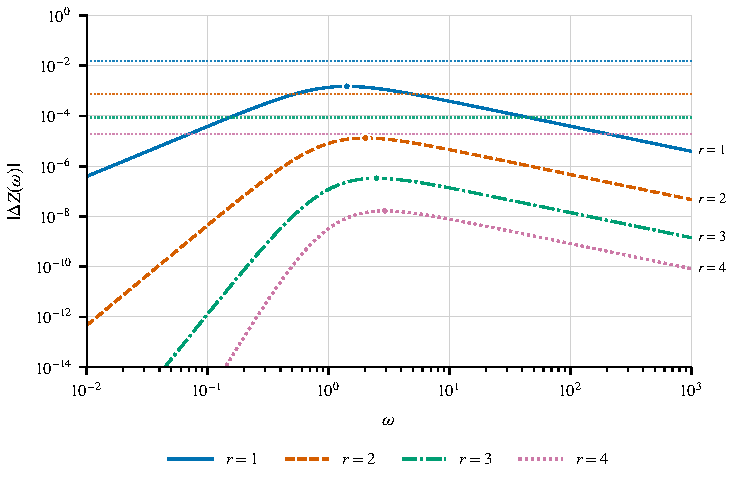
\includegraphics[width=0.86\textwidth]{figures/response_difference.pdf}
\caption{Modulus of the exact response difference \eqref{eq:identity} for the centered pairs with $h=1/8$ and $r=1,\ldots,4$. Markers show the certified maximizers $\omega_*$ of \eqref{eq:maximizer}; dotted lines show the uniform bounds $(2r)!\,2^{1-2r}h^{2r}$. The frequency axis is logarithmic over $[10^{-2},10^{3}]$.}\label{fig:pairs}
\end{figure}

To compare frequency choices at equal total effort on the \emph{same pair}, define
\begin{equation}\label{eq:efficiency}
 A_\Omega=m^{-1}\sum_i|\Delta Z(\omega_i)|^2,\qquad
 e_\Omega=A_\Omega/D_{01}^2.
\end{equation}
Balanced allocation of effort $C$ gives Gaussian information $CA_\Omega/(2\sigma^2)$; an oracle knowing both hypotheses spends everything at $\omega_*$ and gives $CD_{01}^2/(2\sigma^2)$. The latter also bounds the information of policies with $\E_0C_T\le C$, by Lemma~\ref{lem:stopped}'s likelihood calculation. This is the pair-informed benchmark for two-hypothesis discrimination.
Table~\ref{tab:efficiency} lists certified enclosures of $e_\Omega$ for six pairs and two designs. For $r=3$, $h=1/8$, the baseline $\Omega_0=(1,\ldots,6)$ obtains over 35 times the information per unit effort of the high-frequency design $16\Omega_0$, while the pair-informed optimum gains less than a factor $1.622$ over the baseline. Equation~\eqref{eq:identity} also gives $e_\Omega\to e_{\Omega,0}>0$ for every fixed positive design as $h\to0$; the explicit limit and all exact ratios are archived. Equal exponents thus coexist with different information constants: frequency selection changes constants, not the order.

\begin{table}[tb]
\centering
\caption{Same-pair Gaussian information efficiency $e_\Omega$ of \eqref{eq:efficiency} at equal total effort, for the baseline design $\Omega_0=(1,\ldots,6)$ and its scaled version $16\Omega_0$. Intervals are outward rounded. The pair-informed oracle at $\omega_*$ has $e=1$; it knows both hypotheses and is not a spectrum-recovery algorithm.}\label{tab:efficiency}
\begin{tabular}{cccc}\toprule
$r$ & $h$ & $\Omega_0=(1,\ldots,6)$ & $16\Omega_0$ \\\midrule
2 & $1/8$ & $[0.577089, 0.577090]$ & $[0.011924, 0.011925]$ \\
2 & $1/32$ & $[0.574006, 0.574007]$ & $[0.011701, 0.011702]$ \\
3 & $1/8$ & $[0.616696, 0.616697]$ & $[0.017530, 0.017531]$ \\
3 & $1/32$ & $[0.611102, 0.611103]$ & $[0.016847, 0.016848]$ \\
4 & $1/8$ & $[0.640815, 0.640816]$ & $[0.023512, 0.023513]$ \\
4 & $1/32$ & $[0.633893, 0.633894]$ & $[0.021956, 0.021957]$ \\
\bottomrule\end{tabular}
\end{table}

\subsection{Exact ambiguity below the identification threshold}
Sixteen exact positive pairs check Proposition~\ref{prop:frequencycount}: $K=1,\ldots,4$ with unknown calibration at $m=K+1$ for three designs, and with known calibration at $m=K$ for one design. All original channels agree exactly with zero error radius. Each pair has a normalized nonnegative polynomial target with zero reference value and positive alternative value; one further distinct frequency separates it. These exact witnesses instantiate the necessity result with independently checked original-coordinate identities.

For $K=1$, frequencies $(1,2)$ and $(\mu_*,R_*,L_*)=(\delta_0,1/10,1/100)$ give $y=(3/5,49/100,3/10,19/50)$. A different pair is
\[
 \widetilde\mu=\frac{139009}{288000}\delta_{-1/8}
       +\frac{38477}{73984}\delta_{1/8},\qquad
 \widetilde R=\frac1{10}-\frac{767}{650250},\quad
 \widetilde L=\frac1{100}+\frac1{2550}.
\]
Both nuisance values are positive. For $f=x^2/2$, the reference value is zero and the alternative value is $41730113/5326848000>0.00783392$. The original four coordinates are identical; the added frequency $3$ separates them. The alternative has the unrestricted positive mass permitted by $\ThetaAll$. Verification consists of exact zero-noise algebraic identities.

\subsection{Cost bounds and executed stopping paths}
For \eqref{eq:example} with $w=\sigma=10^{-3}$, Lemma~\ref{lem:stopped} gives the expected-effort lower bounds of Table~\ref{tab:cost} at coverage $90\%$, $95\%$, and $99\%$. Eighteen certificates check six pairs and three levels using rational logarithm enclosures. These values are certified analytical lower bounds on expected acquisition effort for any admissible procedure, adaptive or not.

\begin{table}[tb]
\centering
\caption{Certified lower bounds on the expected acquisition effort $\E_0C_T$ from Lemma~\ref{lem:stopped} for the pair in \eqref{eq:example}, $w=\sigma=10^{-3}$. Integer displays are rounded downward. The interval must cover all positive spectra, including the four-atom alternative.}\label{tab:cost}
\begin{tabular}{cr}\toprule
Coverage $1-\alpha$ & Certified lower bound for $\E_0 C_T$\\\midrule
90\% & $>32{,}246{,}594$\\
95\% & $>48{,}614{,}350$\\
99\% & $>82{,}611{,}848$\\
\bottomrule\end{tabular}
\end{table}

The distinct stopping tests use $f=\rho_0^{-1}(2-x)^{-1}$, $\rho_0=D_{(1,2,3,4)}(t)/(1700t^2)$, $\sigma=10^{-3}$, $\alpha=w=1/20$, $b=1/4096$, and numerical allowance $w/4$. References are equal masses at $\pm1/8$ and the three-atom $\mu_0$ above. Fresh seeded Gaussian means are rounded to dyadic centers. Stages start at $(1,2,3,4)$ and add $3/2,5/4$; repeats per frequency are $217,991,4431$. Predeclared radii are $3b_j$ and risk allocations $1/40,1/80,1/160$.
\begin{table}[tb]
\centering
\caption{Two seeded stopping paths at requested width $w=0.05$. Width and excess-budget displays are rounded upward. The common acquisition counts at stages 1, 2, 3 are 868, 5823, 32409 cumulatively.}\label{tab:stopping}
\begin{tabular}{lcrrl}\toprule
Reference & Stage & Outer width & Numerical excess & Decision\\\midrule
Two atoms & 1 & 0.083913616 & 0.000619401 & continue\\
 & 2 & 0.050468900 & 0.000510960 & continue\\
 & 3 & 0.029519810 & 0.000517245 & stop\\
Three atoms & 1 & 0.093536235 & 0.000623884 & continue\\
 & 2 & 0.055185479 & 0.000507675 & continue\\
 & 3 & 0.034075027 & 0.000520947 & stop\\
\bottomrule\end{tabular}
\end{table}

All twelve endpoints are certified, and each weight change preserves the physical target exactly. The two seeded trajectories test the stopping and completion interfaces at the chosen initial scale. The three-atom path exercises completion beyond the nominal two-atom performance class. Statistical coverage follows from the common-event proof in Section~\ref{sec:sequential}; these paths use the target and width stated above. Exact outputs and seeds are archived.

\subsection{Feasibility, relative excess, and verification scope}
The six stage inputs produce strict anchors on quadratic guard grids of 222, 313, and 441 or 442 nodes, with margins above $0.49999999999b_j$. Table~\ref{tab:guard} compares these counts with the calculated first-order sufficient counts of 96,851--387,362; the quadratic guard \eqref{eq:guard} reduces the grid by more than two orders of magnitude at every stage.

\begin{table}[tb]
\centering
\caption{Sufficient guard-grid node counts on the six archived stage inputs: the quadratic guard \eqref{eq:guard} versus the first-order condition. Linear counts are calculated, not executed; all six quadratic grids produced exactly verified strict anchors.}\label{tab:guard}
\begin{tabular}{crrrr}\toprule
 & \multicolumn{2}{c}{Two-atom data} & \multicolumn{2}{c}{Three-atom data} \\
Stage & Linear & Quadratic & Linear & Quadratic \\\midrule
1 & 96,851 & 222 & 96,902 & 222 \\
2 & 193,617 & 313 & 193,716 & 313 \\
3 & 387,169 & 441 & 387,362 & 442 \\
\bottomrule\end{tabular}
\end{table} The certified width brackets satisfy $(\overline W-\underline W)/\underline W<0.01783446$, so the reported intervals enlarge the data-induced information widths by less than $2\%$. Zero-width and nonzero-node-gap controls are included in the archive.

The archive contains 64 range, spectrum, and design tasks, 106 mechanism checks, 16 noiseless-pair checks, and 10 additional altered-input rejections. Independent processes verify raw inputs and certificates; a separate symbolic rebuild checks the noiseless identities. Resource-limited runs return \texttt{UNRESOLVED}. Full tables, seeds, arithmetic primitives, and commands accompany the data.

\section{Conclusions}\label{sec:conclusions}
The analysis determines the frequency information and the measurement effort required to compute calibrated relaxation functionals, and it supplies a finite method that computes them with certified numerical error. Exactly $K+2$ distinct frequencies give uniform noiseless identification of references with at most $K$ atoms among arbitrary positive competitors when resistance and inductance are unknown; known calibration reduces the count to $K+1$. At this threshold a fixed design attains the worst-case functional accuracy order of the entire positive-frequency response, and local target regularity and cluster multiplicity determine that order uniformly through colliding atoms and vanishing masses. The same modulus determines the optimal expected acquisition effort for a prescribed terminal width and confidence.

The continuous range calculation makes the information law computationally accessible. Positive projection gives a strict-feasibility guard, verified primal--dual pairs separate finite optimization from continuum correction, and a finite refinement schedule returns both endpoints at any prescribed numerical excess. Certified width brackets additionally provide absolute--relative accuracy control from the data themselves, and the same calculation drives the sequential design.

Three limitations indicate directions for further work. First, the noise level $\sigma$ and the relaxation-time interval are assumed known. The information bounds of Section~\ref{sec:diameter} extend to any observation family with the two kernel properties isolated in Proposition~\ref{prop:operator}, with different constants, while the numerical and completion results use in addition the rational computability and the Stieltjes uniqueness of the RC kernel; unknown or heteroscedastic noise is not treated. Second, the acquisition design is tuned to a reference class through a certified constant, and the rate is sharp only in order: Section~\ref{sec:experiments} shows that frequency selection still changes the information constant by more than an order of magnitude on the same pair. Third, the computations use synthetic data with exact rational inputs. Applying the certified range calculation to measured impedance data requires a rational error box for the measurements; the predeclared boxes of Section~\ref{sec:sequential} provide one for repeated Gaussian readings, but for instrument data this is a modeling step in its own right.

\section*{Data and software availability}
The accompanying reproducibility archive contains the synthetic inputs, exact certificates, source code, table-generation scripts, and verification commands for the results in Section~\ref{sec:experiments}. The archived inputs are separated from the generating spectra, and the checker routines reconstruct original-coordinate feasibility and continuous dual bounds with exact arithmetic. Machine-readable receipts record the verified quantities and the corresponding file hashes.

\section*{Declarations}
The author declares no conflicts of interest. Generative AI tools were used in developing and checking the mathematical arguments, in literature search, programming, and synthetic-data generation, and in drafting and revising the manuscript. The author verified all results and assumes full responsibility for the content.
\begin{thebibliography}{99}
\bibitem{bland} R.~G. Bland, \emph{New finite pivoting rules for the simplex method}, Math. Oper. Res., 2 (1977), pp.~103--107. \doi{10.1287/moor.2.2.103}.
\bibitem{browngrabovsky} H.~J. Brown and Y. Grabovsky, \emph{On feasibility of extrapolation of completely monotone functions}, SIAM J. Math. Anal., 56 (2024), pp.~7713--7747. \doi{10.1137/24M1652325}.
\bibitem{cailow} T.~T. Cai and M.~G. Low, \emph{An adaptation theory for nonparametric confidence intervals}, Ann. Statist., 32 (2004), pp.~1805--1840. \doi{10.1214/009053604000000049}.
\bibitem{castro} R.~M. Castro, \emph{Adaptive sensing performance lower bounds for sparse signal detection and support estimation}, Bernoulli, 20 (2014), pp.~2217--2246. \doi{10.3150/13-BEJ555}.
\bibitem{ciucci} F. Ciucci and C. Chen, \emph{Analysis of electrochemical impedance spectroscopy data using the distribution of relaxation times: A Bayesian and hierarchical Bayesian approach}, Electrochim. Acta, 167 (2015), pp.~439--454. \doi{10.1016/j.electacta.2015.03.123}.
\bibitem{deboor} C. de Boor, \emph{Divided differences}, Surv. Approx. Theory, 1 (2005), pp.~46--69.
\bibitem{donoho} D.~L. Donoho, \emph{Statistical estimation and optimal recovery}, Ann. Statist., 22 (1994), pp.~238--270. \doi{10.1214/aos/1176325367}.
\bibitem{eftekhari} A. Eftekhari, J. Tanner, A. Thompson, B. Toader, and H. Tyagi, \emph{Sparse non-negative super-resolution---simplified and stabilised}, Appl. Comput. Harmon. Anal., 50 (2021), pp.~216--280. \doi{10.1016/j.acha.2019.08.004}.
\bibitem{ettehad} M. Ettehad and S. Foucart, \emph{Instances of computational optimal recovery: Dealing with observation errors}, SIAM/ASA J. Uncertain. Quantif., 9 (2021), pp.~1438--1456. \doi{10.1137/20M1328476}.
\bibitem{grid} A. Flinth, F. de Gournay, and P. Weiss, \emph{Grid is Good: Adaptive refinement algorithms for off-the-grid total variation minimization}, Open J. Math. Optim., 6 (2025), article~3. \doi{10.5802/ojmo.39}.
\bibitem{garivier} A. Garivier and E. Kaufmann, \emph{Optimal best arm identification with fixed confidence}, Proc. Mach. Learn. Res., 49 (2016), pp.~998--1027. \url{https://proceedings.mlr.press/v49/garivier16a.html}.
\bibitem{grabovsky} Y. Grabovsky, \emph{Reconstructing Stieltjes functions from their approximate values: A search for a needle in a haystack}, SIAM J. Appl. Math., 82 (2022), pp.~1135--1166. \doi{10.1137/21M1392279}.
\bibitem{howard} S.~R. Howard, A. Ramdas, J. McAuliffe, and J. Sekhon, \emph{Time-uniform, nonparametric, nonasymptotic confidence sequences}, Ann. Statist., 49 (2021), pp.~1055--1080. \doi{10.1214/20-AOS1991}.
\bibitem{jansson} C. Jansson, \emph{Rigorous lower and upper bounds in linear programming}, SIAM J. Optim., 14 (2004), pp.~914--935. \doi{10.1137/S1052623402416839}.
\bibitem{karlinstudden} S. Karlin and W.~J. Studden, \emph{Tchebycheff Systems: With Applications in Analysis and Statistics}, Pure Appl. Math. XV, Interscience, New York, 1966.
\bibitem{kaufmann} E. Kaufmann, O. Capp\'e, and A. Garivier, \emph{On the complexity of best-arm identification in multi-armed bandit models}, J. Mach. Learn. Res., 17 (2016), article~1, pp.~1--42. \url{https://jmlr.org/papers/v17/kaufman16a.html}.
\bibitem{kreinnudelman} M.~G. Kre\u{\i}n and A.~A. Nudel'man, \emph{The Markov Moment Problem and Extremal Problems}, Transl. Math. Monogr. 50, Amer. Math. Soc., Providence, RI, 1977.
\bibitem{knpu} D. Krieg, E. Novak, L. Plaskota, and M. Ullrich, \emph{Noisy nonlinear information and entropy numbers}, J. Fourier Anal. Appl., 32 (2026), article~36. \doi{10.1007/s00041-026-10249-z}.
\bibitem{knu} D. Krieg, E. Novak, and M. Ullrich, \emph{On the power of adaption and randomization}, Forum Math. Sigma, 13 (2025), e152. \doi{10.1017/fms.2025.10101}.
\bibitem{liuammari} P. Liu and H. Ammari, \emph{Super-resolution of positive near-colliding point sources}, preprint, arXiv:2212.00536, 2022. \url{https://arxiv.org/abs/2212.00536}.
\bibitem{nguyen} H. Nguyen, D. Le, A. Rinaldo, and N. Ho, \emph{On the geometry of separation in finite Gaussian mixtures}, preprint, arXiv:2606.16179, 2026. \url{https://arxiv.org/abs/2606.16179}.
\bibitem{orazem} M.~E. Orazem and B. Tribollet, \emph{Electrochemical Impedance Spectroscopy}, 2nd ed., Wiley, Hoboken, NJ, 2017.
\bibitem{pages} G. Pag\`es and B. Wilbertz, \emph{Intrinsic stationarity for vector quantization: Foundation of dual quantization}, SIAM J. Numer. Anal., 50 (2012), pp.~747--780. \doi{10.1137/110827041}.
\bibitem{papp} D. Papp, \emph{Semi-infinite programming using high-degree polynomial interpolants and semidefinite programming}, SIAM J. Optim., 27 (2017), pp.~1858--1879. \doi{10.1137/15M1053578}.
\bibitem{schmid} J. Schmid and M. Poursanidis, \emph{Approximate solutions of convex semi-infinite optimization problems in finitely many iterations}, preprint, arXiv:2105.08417v2, 2022. \url{https://arxiv.org/abs/2105.08417}.
\bibitem{sovljanski} V. Sovljanski, M. Paolone, S. Tant, and D.~P. Sainflou, \emph{Optimizing experiments for accurate battery circuit parameters estimation: Reduction and adjustment of frequency set used in electrochemical impedance spectroscopy}, preprint, arXiv:2501.06112, 2025. \url{https://arxiv.org/abs/2501.06112}.
\bibitem{stark} P.~B. Stark, \emph{Inference in infinite-dimensional inverse problems: Discretization and duality}, J. Geophys. Res. Solid Earth, 97 (1992), pp.~14055--14082. \doi{10.1029/92JB00739}.
\bibitem{wan} T.~H. Wan, M. Saccoccio, C. Chen, and F. Ciucci, \emph{Influence of the discretization methods on the distribution of relaxation times deconvolution: Implementing radial basis functions with DRTtools}, Electrochim. Acta, 184 (2015), pp.~483--499. \doi{10.1016/j.electacta.2015.09.097}.
\bibitem{wasilwoz} G.~W. Wasilkowski and H. Wo\'zniakowski, \emph{The power of standard information for multivariate approximation in the randomized setting}, Math. Comp., 76 (2007), pp.~965--988. \doi{10.1090/S0025-5718-06-01944-2}.
\bibitem{wuyang} Y. Wu and P. Yang, \emph{Optimal estimation of Gaussian mixtures via denoised method of moments}, Ann. Statist., 48 (2020), pp.~1981--2007. \doi{10.1214/19-AOS1873}.
\end{thebibliography}

\end{document}
